%% 방법 논문 초안 v0.3의 한국어 번역본(검토·공유용). 제출본은 영어 main.tex. 이전 판: main_ko_v0.1.tex, main_ko_v0.2.tex.
%% Overleaf: Main document = main_ko.tex, Compiler = pdfLaTeX (한글 글꼴 오류 시 XeLaTeX).
\documentclass[twocolumn,10pt]{article}
\usepackage[letterpaper,margin=0.75in,columnsep=0.25in]{geometry}
\usepackage{kotex}
\usepackage[round]{natbib}
\usepackage{graphicx}
\usepackage{amsmath}
\usepackage{amssymb}
\usepackage{amsthm}
\usepackage{booktabs}
\usepackage{xcolor}
\usepackage[small]{caption}
\usepackage{url}
\usepackage{algorithm}
\usepackage{algpseudocode}

\newtheorem{proposition}{명제}
\newtheorem{lemma}{보조정리}
\newtheorem{assumption}{가정}
\newtheorem{definition}{정의}
\theoremstyle{remark}
\newtheorem{remark}{비고}

\newcommand{\todo}[1]{\textcolor{red}{[TODO: #1]}}
\newcommand{\tbd}{\textcolor{red}{TBD}}
\newcommand{\pilot}{\textsuperscript{\textcolor{gray}{$\dagger$}}}
\newcommand{\sg}{\operatorname{sg}}
\newcommand{\JS}{\operatorname{JS}}
\newcommand{\KL}{\operatorname{KL}}
\newcommand{\ours}{PGCT}
\floatname{algorithm}{알고리즘}

\title{Probe-Gated Critic Transfer:\\ 선택적 critic 공유를 위한 국소 팀원 추론\\ (다중 agent 강화학습)}
\author{익명 제출 (한국어 번역본)}
\date{}

\begin{document}
\maketitle

\begin{abstract}
공유된 환경의 agent들이 서로 다른 목표를 가진 잠재 팀에 속할 때, 팀 안에서 가치 추정을 공유하면 학습이 빨라질 수 있지만 agent는
누가 팀원인지 거의 알지 못한다. 우리는 Probe-Gated Critic Transfer(\ours{})를 연구한다. 이웃 agent들은 미리 합의한 고정 probe 관측 집합에서
행동 분포를 비교하고, 평활화한 Jensen--Shannon divergence에 임계값을 적용해 국소 팀원을 추론하며, 추론한 팀원의 critic을 probe 입력에서
distillation한다. 행동 유사성이 일반적으로 같은 목표를 뜻하지 않고, 같은 목표가 호환되는 가치 함수를 뜻하지도 않으므로, 우리는 조건을 명시한다.
probe divergence가 유계·대칭·결합 볼록이며 그 제곱근이 pseudometric임을 보인다. 분리 마진이 추정 오차의 두 배보다 크면 임계값이 국소 팀 관계를
정확히 복원하며, 그 오차를 update당 정책 변화로 한정한다. critic distillation은 critic 출력에 대해 강볼록이어서 잘못된 donor가 receiver를 가치 차이의
$\lambda/(c+\lambda)$배 이하로만 치우치게 한다. 또 팀이 유도하는 결정 문제가 일치하면 같은 입력에 대한 반응을 비교하는 어떤 방법으로도 팀을 가를 수 없다.
팀 대칭 창고 과제가 이 마지막 경우에 해당한다. seed 1개 예비 실행에서 \ours{}는 팀을 가로질러 연결했지만, 독립 PPO보다(평균 처리량 12\%, 최종 18\% 높음)
그리고 무차별 공유보다 나았다. 분리 조건이 성립할 수 있는 목표 분리 과제는 평가 중이다 \todo{E1-F, seed, 전이량 통제 gate}.
\end{abstract}

\section{서론}
많은 다중 agent 시스템은 공유된 공간에서 서로 다른 목표를 추구하는 집단으로 이루어진다. 서로 다른 고객사의 창고 로봇, 서로 다른 운송사의 차량, 여러 팀의
선수들이 그렇다. 집단 안에서는 학습한 것(파라미터, 경험, 가치 추정)을 공유하는 것이 다중 agent 강화학습(MARL)의 표본 효율을 높이는 효과적인 방법이다
\cite{christianos2020seac,christianos2021seps}. 집단 사이에서는 같은 지식이 다른 목표를 묘사할 수 있다. 집단 소속이 숨겨져 있으면 각 agent는 세 가지 다른
질문에 답해야 한다. \emph{(Q1) 누가 내 팀원인가?} \emph{(Q2) 누구의 critic이 내 학습을 돕는가?} \emph{(Q3) Q1의 답은 언제 Q2의 좋은 답인가?}

Q1에 대한 분산적 답으로 행동을 비교하는 방법이 있다. 미리 합의한 같은 probe 관측을 평가하는 두 agent는 경험을 교환하지 않고 행동 분포를 비교할 수 있다.
이것이 Probe-Gated Critic Transfer(\ours{})의 아이디어다. 이웃들은 probe 응답의 평활화한 Jensen--Shannon(JS) divergence에 임계값을 적용해 국소 팀원을 추론하고,
추론한 팀원의 critic을 probe 입력에서 distillation한다. 이 아이디어는 일반적으로는 성립하지 않는 두 고리에 기댄다. 행동 유사성은 같은 목표를 뜻하지 않는다.
다른 목표가 같은 행동을 낳을 수 있고, 팀원이 다른 역할을 맡을 수 있으며, 학습되지 않은 정책은 모두 비슷해 보인다. 정책은 보상을 식별하지 못한다
\cite{ng2000irl}. 또 같은 목표가 호환되는 가치 함수를 뜻하지 않는다. 개인 보상에서는 팀원끼리 같은 과제를 두고 경쟁하고 숙련도도 다르다.

우리는 이 고리들을 가정하는 대신 언제 성립하는지 명시하고 검증한다. 기여는 다음과 같다.
\begin{itemize}
  \item \textbf{방법.} 공유 probe 집합에 대한 모델 출력만 교환하는 국소·무라벨 팀원 추론 및 critic 전이 방법 \ours{}와 재현에 필요한 모든 구현 세부(\ref{sec:method}절).
  \item \textbf{분석.} probe divergence의 성질, 분리 마진 아래 정확한 국소 복원, update당 정책 변화에 묶인 추정 오차 한계, 출력 공간에서 distillation의 강볼록성과
    잘못된 donor의 편향 한계, 정책 유사성이 가치 유사성을 보장하지 않는다는 반례, 유도 결정 문제가 일치하는 팀의 식별 불가능성(\ref{sec:analysis}절).
  \item \textbf{평가 설계.} 팀의 행동적 식별 가능성과 팀 내 critic 호환성이라는 두 축에 환경을 배치하고, 팀 선택과 전이량을 분리하는 baseline을 둔다(\ref{sec:setup}절).
  \item \textbf{예비 증거.} 분석이 팀 식별 불가능을 예측하는 팀 대칭 과제에서, \ours{}는 실제로 팀을 복원하지 못했지만 seed 1개 실행에서 독립 학습과 무차별
    공유보다 나았다(\ref{sec:results}절). \todo{목표 분리 과제; seed; 전이량 통제 gate}
\end{itemize}

\section{관련 연구}
\textbf{선택적 공유.} SePS는 학습 전에 transition 인코딩으로 agent를 군집화하고 군집 안에서 파라미터를 공유한다~\cite{christianos2021seps}. MADPS는 agent 정책 사이의
거리를 측정해 파라미터 공유를 온라인으로 조정한다~\cite{hu2024madps}. HetDPS는 정책 이질성과 목표 이질성을 포함한 여러 이질성을 구분하고 그에 따라 동적으로
공유한다~\cite{hu2026hetdps}. SEAC는 importance weighting으로 경험을 공유한다~\cite{christianos2020seac}. 따라서 정책 거리로 공유 상대를 정하는 것 자체는 새롭지 않다.
\ours{}의 차이는 (i) 중앙 군집화 없이 현재 통신 이웃 사이에서 국소·온라인으로 상대를 고르는 것, (ii) 공유 궤적이나 파라미터 대신 고정 probe 집합으로 비교하는 것,
(iii) critic 예측만 전이하고 actor는 비공개 경험으로 학습하는 것의 조합에 있다. 개별 요소의 새로움을 주장하지 않으며, 그 조합이 언제 정당한지 분석한다.

\textbf{분산 critic과 distillation.} 네트워크 actor-critic 방법은 통신 그래프 위에서 critic 파라미터를 합의로 이끌며, 선형 함수 근사와 네트워크 평균 목적에서 수렴이
보장된다~\cite{zhang2018networked}. 이 보장은 개인 보상·비선형인 우리 설정으로 옮겨지지 않는다. \ours{}는 probe 입력에서의 distillation으로 전이한다
\cite{rusu2016policy}.

\textbf{역할, 독립 학습, 식별 가능성.} 역할과 팀은 다른 잠재 변수이며, 역할 기반 방법은 행동의 효과로 역할을 발견한다~\cite{wang2021rode}. 독립 PPO는 협력 MARL의 강한
baseline이고~\cite{schulman2017ppo,dewitt2020ippo}, MAPPO는 중앙 critic을 쓴다~\cite{yu2022mappo}. 정책이 보상을 결정하지 않는다는 것은 역강화학습의 고전적 결과이며
\cite{ng2000irl}, 우리의 식별 불가능성 결과는 그 팀 수준 사례다. 보고는 \cite{agarwal2021precipice}를 따른다.

\section{문제 설정}
\label{sec:setting}
agent $i\in\{1,\dots,N\}$, 관측 $o_i^t$, 행동 $a_i^t\in\mathcal{A}$, 개인 보상 $r_i^t$를 가진 부분관측 확률 게임을 고려한다. 각 agent는 목표를 정하는 잠재 팀
$z_i\in\{1,\dots,K\}$에 속한다. agent는 자기 목표는 알지만 다른 agent의 $z_j$는 모른다. 통신 범위 안의 agent는 시간에 따라 바뀌는 이웃 $\mathcal{N}_i(t)$를 이룬다.
학습 전 모든 agent는 같은 probe 집합을 받고, 학습 중 이웃끼리 probe 입력에 대한 행동 확률과 critic 예측을 교환할 수 있다. 관측, 경험, 파라미터, 팀 라벨은 교환하지 않는다
(교환하는 출력이 정책에 관한 정보를 일부 드러내므로 프라이버시는 주장하지 않는다). 각 agent는 PPO로 recurrent actor $\pi_i$와 critic $V_i$를 학습한다.

\begin{definition}[국소 팀 관계]
시점 $t$에서 agent $i$의 국소 팀 관계는 $\mathcal{T}_i(t)=\{j\in\mathcal{N}_i(t): z_j=z_i\}$이다. 방법의 추정 $\hat{\mathcal{T}}_i(t)$가 이와 같으면 복원했다고 한다.
\end{definition}

\begin{definition}[전이 효용]
같은 학습 상태 $\Theta_n$에서 donor $j$를 쓰는 update와 독립 update를 짝지었을 때, 전이 효용은
$U_{i\leftarrow j}=\mathbb{E}[J_i(\Theta^{i\leftarrow j}_{n,+})-J_i(\Theta^{i}_{n,+})]$이다. $J_i$는 agent $i$의 평가 return이다~\cite{agarwal2021precipice}.
Q1은 $\mathcal{T}_i$를, Q2는 $U_{i\leftarrow j}>0$인 donor를 묻는다.
\end{definition}

\section{Probe-Gated Critic Transfer}
\label{sec:method}
\textbf{Probe 집합.} 모든 agent는 학습 전에 환경 배치에서 결정적 규칙으로 생성한 단일 step 관측 집합 $\mathcal{Q}=\{q_m\}_{m=1}^{M}$을 가진다. probe는 recurrent 상태 0,
action mask 없이 평가하므로 질의는 forward 한 번이고 학습 궤적을 바꾸지 않는다.

\begin{assumption}[Probe 비교 가능성]
\label{as:comparability}
모든 probe $q_m$은 모든 agent에게 유효한 관측이며, 관측하는 agent 자신의 목표를 기준으로 상황을 모든 agent에게 같은 방식으로 표현한다.
\end{assumption}
팀 기준 관측 채널에서는 같은 텐서가 모든 agent에게 ``내 요청 선반'', ``내 목표''를 뜻한다. 다른 팀의 목표를 보여 주는 probe는 이 가정을 어기므로 구성 단계에서
제외한다(\ref{sec:setup}절).

\textbf{Probe divergence.} $p_i^m=\pi_i(\cdot\mid q_m,h=0)$라 하자. $P$ update마다 이웃은 $\{p_i^m\}_m$을 교환하고 다음을 계산한다.
\begin{equation}
  D_{ij}=\frac{1}{M}\sum_{m=1}^{M}\JS(p_i^m,p_j^m),\quad
  \JS(p,q)=\tfrac12\KL(p\Vert\tfrac{p+q}{2})+\tfrac12\KL(q\Vert\tfrac{p+q}{2})
  \label{eq:div}
\end{equation}
자연로그를 쓰므로 $D_{ij}\in[0,\ln 2]$이고 단위는 nats다. $D_{ij}$는 JS \emph{divergence}이며, 그 제곱근이 JS \emph{distance}다.

\textbf{평활화와 gate.} 첫 측정이 $\bar D_{ij}\gets D_{ij}$로 초기화하고, 이후 측정은 $i$와 $j$가 이웃인 동안에만 $\bar D_{ij}\gets(1-\beta)\bar D_{ij}+\beta D_{ij}$로
갱신한다. 서로의 범위를 벗어나면 $\bar D_{ij}$와 측정 횟수 $n_{ij}$는 유지하되 전이는 하지 않는다. $U_0$ update의 warm-up 뒤 agent $i$는 다음을 추론한다.
\begin{equation}
  \hat{\mathcal{T}}_i(t)=\{j\in\mathcal{N}_i(t): n_{ij}\ge n_{\min},\ \bar D_{ij}<\tau\}
\end{equation}

\textbf{팀 내 critic distillation.} $j\in\hat{\mathcal{T}}_i(t)$에 대해 $\alpha_{ij}=1/|\hat{\mathcal{T}}_i(t)|$로 두고(집합이 비면 peer 항 없음), agent $i$는 다음을 최소화한다.
\begin{equation}
  \mathcal{L}_i=\mathcal{L}^{\mathrm{PPO}}_i+\lambda\sum_{j\in\hat{\mathcal{T}}_i(t)}\alpha_{ij}\,
  \frac{1}{M_{\mathrm{d}}}\sum_{m=1}^{M_{\mathrm{d}}}\big(V_i(q^{\mathrm{d}}_m)-\sg[V_j(q^{\mathrm{d}}_m)]\big)^2
  \label{eq:loss}
\end{equation}
$\mathcal{L}^{\mathrm{PPO}}_i$는 최소화할 PPO 손실(음의 clipped surrogate, $c$배 가치 손실, entropy 보너스 차감)이고, $\sg$는 stop-gradient이며, donor 값은 update 시작
시점에 고정한다. 한 쌍의 두 방향이 같은 update에서 함께 활성일 수 있고, 각 receiver는 상대의 update 전 값을 쓴다. 기본 변형은 probe 집합 자체에서 distillation하고,
\ours{}-v2는 추론용 집합에는 팀을 가르는 상태만 두고 모든 과제 단계를 덮는 별도 distillation 집합을 쓴다.

\textbf{비용.} probe 라운드마다 agent당 forward $M$번, 쌍마다 확률 $M|\mathcal{A}|$개를 교환한다. 전이가 활성이면 값 $M_{\mathrm{d}}$개가 더해진다. $M=48$,
$|\mathcal{A}|=5$, $P=5$, rollout 1{,}024 step이면 환경 5{,}120 step마다 쌍당 240개다.

\begin{algorithm}[t]
\caption{agent $i$의 \ours{}}
\label{alg:pgct}
\begin{algorithmic}[1]
\State $\pi_i,V_i$ 초기화; 모든 $j$에 대해 $\bar D_{ij}$ 미정, $n_{ij}\gets 0$
\For{update $u=1,2,\dots$}
  \State $\pi_i$로 rollout 수집; 자기 보상으로 PPO target 계산
  \If{$u\bmod P=0$}
    \For{$j\in\mathcal{N}_i(t)$}
      \State $\mathcal{Q}$에서 $\{p^m\}$ 교환; $D_{ij}$ 계산(식~\ref{eq:div})
      \State $n_{ij}=0$이면 $\bar D_{ij}\gets D_{ij}$, 아니면 $(1-\beta)\bar D_{ij}+\beta D_{ij}$; $n_{ij}\gets n_{ij}+1$
    \EndFor
  \EndIf
  \State $u>U_0$이면 $\hat{\mathcal{T}}_i\gets\{j\in\mathcal{N}_i(t):n_{ij}\ge n_{\min},\bar D_{ij}<\tau\}$, 아니면 $\emptyset$
  \State $j\in\hat{\mathcal{T}}_i$로부터 update 전 $V_j(q^{\mathrm{d}}_m)$ 수신
  \State $\mathcal{L}_i$(식~\ref{eq:loss})로 $\pi_i,V_i$ 갱신; $\hat{\mathcal{T}}_i=\emptyset$이면 peer 항 생략
\EndFor
\end{algorithmic}
\end{algorithm}

\section{분석}
\label{sec:analysis}
증명은 부록 A에 있다. $\Delta(\mathcal{A})$는 행동에 대한 확률 단체다.

\textbf{Probe divergence.} JS divergence는 gate 통계량으로만 쓰이며 gradient가 흐르지 않는다. 중요한 것은 분포 공간에서의 성질이다.
\begin{proposition}[성질]
\label{prop:properties}
(a) $0\le D_{ij}\le\ln 2$, $D_{ij}=D_{ji}$이고, $D_{ij}=0$은 모든 $m$에 대해 $p_i^m=p_j^m$과 동치다.
(b) $D_{ij}$는 $(\{p_i^m\}_m,\{p_j^m\}_m)$에 대해 결합 볼록이다.
(c) $d_{ij}=\sqrt{D_{ij}}$는 정책 위의 pseudometric이며, 특히 $d_{ik}\le d_{ij}+d_{jk}$이다.
\end{proposition}
\begin{remark}
$D_{ij}$를 최소화하지 않으므로 신경망 파라미터에 대한 비볼록성은 최적화에 영향을 주지 않는다. gate가 일으킬 수 있는 불안정은 다른 종류다. hard threshold 때문에 donor
집합이 $\bar D_{ij}$의 불연속 함수가 되어, $\tau$ 근처의 추정값이 연속 update 사이에 gate를 뒤집을 수 있다. 명제~\ref{prop:recovery}와 \ref{prop:tracking}는 이것이 추론
관계를 바꿀 수 없는 조건을 정량화한다. (c)는 근사적 추이성을 준다. $i$가 $j$와, $j$가 $k$와 가까우면 $i$는 $k$와 가깝다.
\end{remark}

\textbf{임계값은 언제 팀을 복원하는가?}
\begin{assumption}[분리]
\label{as:separation}
update $n$에서 현재 이웃 쌍에 대한 $\delta_{\mathrm{in}}(n)=\max_{z_i=z_j}D_{ij}(n)$과 $\delta_{\mathrm{out}}(n)=\min_{z_i\ne z_j}D_{ij}(n)$이
$\Delta(n)=\delta_{\mathrm{out}}(n)-\delta_{\mathrm{in}}(n)>0$을 만족한다.
\end{assumption}
\begin{proposition}[정확한 국소 복원]
\label{prop:recovery}
가정~\ref{as:separation} 아래, 모든 이웃 쌍에 대해 $|\bar D_{ij}(n)-D_{ij}(n)|\le\epsilon$, $2\epsilon<\Delta(n)$,
$\tau\in(\delta_{\mathrm{in}}+\epsilon,\delta_{\mathrm{out}}-\epsilon)$이고 warm-up과 최소 횟수를 만족하면, 모든 $i$에 대해 $\hat{\mathcal{T}}_i(n)=\mathcal{T}_i(n)$이다. 특히
추론 관계는 대칭이며 잘못된 donor는 쓰이지 않는다.
\end{proposition}
명제 자체는 간단하다. 가치는 측정해야 할 두 양, 마진 $\Delta$와 오차 $\epsilon$을 명시한다는 데 있다. probe 응답은 결정적이므로 $\epsilon$은 표본 잡음이 아니라 측정 사이에
정책이 바뀌고 평균이 뒤처지는 데서 온다.
\begin{lemma}[변화량]
\label{lem:drift}
연속한 두 측정 사이에 $i$와 $j$의 모든 probe 응답이 대칭화 KL로 $\KL(p\Vert p')+\KL(p'\Vert p)\le\kappa$ 이하로 바뀌면, $|d_{ij}'-d_{ij}|\le\sqrt{\kappa}$이고
$|D_{ij}'-D_{ij}|\le2\sqrt{\kappa\ln 2}$이다.
\end{lemma}
\begin{proposition}[추적 오차]
\label{prop:tracking}
쌍의 모든 측정에서 $|D_{ij}(n)-D_{ij}(n-1)|\le\rho$이면, 첫 측정으로 초기화한 평활 추정은 $|\bar D_{ij}(n)-D_{ij}(n)|\le\frac{1-\beta}{\beta}\rho$를 만족한다. 따라서
$2\frac{1-\beta}{\beta}\rho<\Delta(n)$이면 명제~\ref{prop:recovery}가 적용된다.
\end{proposition}
PPO의 clipped 목적은 방문 상태에서 update당 평균 KL을 작게 유지하므로 작은 $\kappa$를 뒷받침하지만, probe 입력에서의 KL을 묶지는 않는다. 그래서 보조정리~\ref{lem:drift}는
충분조건이며 $\rho$는 직접 측정한다 \todo{checkpoint에서 실측 $\rho$와 $\Delta$}. $\beta=0.35$에서 $(1-\beta)/\beta$는 1.86이다. $\beta$가 크면 빨리 따라가지만 덜 평균하며,
gate 깜빡임에는 이중 임계값(hysteresis)이 표준적인 대처다.

\textbf{잘못된 donor의 비용은?} 하나의 probe 입력 $q$에서 critic을 자유 출력 $v$, 국소 회귀 target $y$(예: receiver 자신의 return 추정), donor 값 $v_j$로 이상화한다.
\begin{proposition}[출력 공간의 distillation]
\label{prop:bias}
$\sum_j\alpha_{ij}=1$일 때 $f(v)=c(v-y)^2+\lambda\sum_j\alpha_{ij}(v-v_j)^2$은 $2(c+\lambda)$-강볼록이고 최소점은
$v^\star=\frac{cy+\lambda\sum_j\alpha_{ij}v_j}{c+\lambda}$이다. $\hat{\mathcal{T}}_i$의 donor가 $z_j=z_i$이면 $|v_j-y|\le\eta$, 아니면 $|v_j-y|\le\Gamma$를 만족하고 잘못된
donor의 가중치 합이 $a_{\mathrm{w}}$이면 $|v^\star-y|\le\frac{\lambda}{c+\lambda}\big((1-a_{\mathrm{w}})\eta+a_{\mathrm{w}}\Gamma\big)$이다.
\end{proposition}
가치 손실 계수 $c=0.5$, $\lambda=0.01$에서 $\lambda/(c+\lambda)$는 약 0.02다. 이 이상화에서 distillation은 critic을 donor 쪽으로 볼록 결합만큼 당긴다. 명제~\ref{prop:recovery}
아래에서는 $a_{\mathrm{w}}=0$이다. 이 이상화는 신경망이 입력 사이에 파라미터를 공유한다는 점과 $c$가 probe가 아닌 rollout 상태에 걸린다는 점을 무시한다. 파라미터 수준에서는
$\langle\nabla\mathcal{L}^V_i,\nabla\mathcal{L}^D_{i\leftarrow j}\rangle<0$일 때 peer 항이 가치 손실과 충돌할 수 있으며, 이를 진단 지표로 관찰할 것을 제안한다
\todo{gradient 정렬 측정}.

\textbf{팀 관계는 언제 호환성의 좋은 대리 지표인가?}
\begin{proposition}[정책 유사성은 가치 유사성을 묶지 않는다]
\label{prop:counter}
모든 probe에서 $D_{ij}=0$이면서 $|V_i-V_j|=1/(1-\gamma)$인 두 agent가 존재한다.
\end{proposition}
이 반례는 Q1만으로 Q2에 답할 수 없음을 명시한다. 호환성은 측정해야 한다.

\textbf{팀은 언제 식별 가능한가?} 다른 agent의 정책을 고정하면 agent $i$는 자기 관측 위의 단일 agent 결정 문제를 마주한다. 모든 기억 없는 관측-행동 사상 $\mu$에 대해,
$i$가 $\mu$로 행동할 때 겪는 관측--보상 열의 분포가 $j$가 $\mu$로 행동할 때와 같으면 두 agent의 문제가 \emph{일치한다}고 하자.
\begin{proposition}[팀 불변 결정 문제에서의 식별 불가능성]
\label{prop:nonid}
서로 다른 팀 agent들이 유도하는 결정 문제가 관측의 함수로서 일치하면, 기억 없는 정책 안에서 한 팀에 최적인 모든 관측-행동 사상은 다른 팀에도 최적이다. 최적 사상이
유일하면 목표 최적 정책은 모든 쌍에서 $D_{ij}=0$을 만족하므로 $\Delta=0$이고 어떤 임계값도 팀을 가르지 못한다. 이때 probe 응답의 차이는 역할이나 학습 진행 같은 목표 외
요인을 반영한다.
\end{proposition}
팀 기준 관측과 거울 대칭 과제가 함께 있으면 정확히 이 경우가 된다. 반대로 관측에 팀에 따라 의미가 바뀌지 않는 양(예: agent의 절대 위치)이 있고 팀의 목표가 다르면,
유도 결정 문제가 달라져 명제~\ref{prop:nonid}가 적용되지 않는다.

\section{실험 설계}
\label{sec:setup}
\textbf{두 축 위의 환경.} 다중 로봇 창고~\cite{papoudakis2021benchmarking}의 두 팀 변형을 $11\times10$ 맵에서 agent 4명으로 쓴다(agent 1, 3은 빨강 팀, 2, 4는 파랑 팀).
각 팀은 항상 요청 선반 2개와 자기 목표를 가지며, 각 팀 선반의 절반은 상대 구역에 있다. 관측은 팀 기준 채널을 가진 자기 중심 $11\times11$ semantic grid와 절대 위치를
포함한 ego feature다. 보상은 개인별이다.

\begin{table}[t]
\centering
\small
\resizebox{\columnwidth}{!}{%
\begin{tabular}{lcc}
\toprule
 & 팀 내 critic 호환 & 호환되지 않음 \\
\midrule
행동으로 팀 식별 가능 & E1-F + 팀 보상(계획) & E1-F(개인 보상)? \\
식별 불가능 & -- & E1(측정됨) \\
\bottomrule
\end{tabular}}
\caption{분석의 두 축에 놓은 환경. E1: 명제~\ref{prop:nonid}로 식별 가능성이 배제되고, 팀 내 호환성이 팀 간보다 낮게 측정됨. E1-F: 식별 가능성이 기대되며 호환성은 측정 예정.
\todo{측정 후 E1-F 위치 확정}}
\label{tab:axes}
\end{table}

\begin{itemize}
  \item \textbf{E1(팀 대칭).} 목표가 맵 아래 가운데에 붙어 있다. 팀 기준 채널에서 두 팀은 같은 결정 문제를 마주하므로 명제~\ref{prop:nonid}가 적용된다.
  \item \textbf{E1-F(목표 분리).} 목표가 맵 아래 양쪽 모서리에 있다. 선반을 든 agent는 자기 모서리로 가야 하며, 관측에 절대 위치가 있으므로 결정 문제가 달라지고 팀이
    식별 가능할 수 있다.
  \item \textbf{E1-F + 팀 보상}(계획): 배송·반납 보상을 팀 안에서 공유해 팀원이 같은 가치 target을 갖게 한다.
\end{itemize}

\textbf{Probe 집합.} canonical 집합은 pickup, 배송, 반납을 덮는 48개 상태다. v2 추론 집합은 agent가 요청 선반을 들고 있고 \emph{어느 팀의 목표도} 보이지 않는 48개 상태로,
같은 입력이 모든 agent에게 유효하고(가정~\ref{as:comparability}) 행동이 자기 팀의 배송 위치에 달려 있다. v2 distillation 집합은 과제 단계별로 균형 잡힌 64개 상태다. 모든
probe는 학습 환경에서 실현하고 검증한다.

\textbf{방법.} IPPO(전이 없음), All-peer(모든 이웃), Oracle-team(이웃 중 정답 팀원; 특권 참조 기준이며 상한이 아님), \ours{}, \ours{}-v2. \emph{누구와} 공유하는지와
\emph{얼마나} 공유하는지를 분리하기 위해, \ours{}의 실제 update당 donor 수만큼 이웃 중에서 무작위로 donor를 뽑는 Random-gated 전이와 전이량을 맞춘 Oracle을 추가한다
\todo{구현 및 실행}. 같은 seed에서 모든 방법은 비트 단위로 같은 가중치에서 시작하며 donor 집합만 다르다. \ours{}는 $P=5$, $\beta=0.35$, $\tau=0.12$ nats, $U_0=100$,
$n_{\min}=8$, $\lambda=0.01$, $c=0.5$를 쓴다(부록 B).

\textbf{지표.} \emph{학습}: 배송 시작(3점 이동평균이 episode당 배송 1개에 처음 도달한 step), 학습 중 평균 배송, 최종 배송(마지막 평가 5회), 학습한 agent 수.
\emph{추론}: 실제 update에서 $\mathcal{T}_i$ 대비 $\hat{\mathcal{T}}_i$의 정밀도·재현율·F1, checkpoint에서 $D_{ij}$의 같은 팀 AUROC, 실측 마진 $\Delta$와 변화량 $\rho$.
\emph{호환성}: receiver의 critic을 팀원과 섞을 때와 팀원이 아닌 agent와 섞을 때의 가치 오차 감소. \emph{전이}: update당 실제 donor 수, 팀 내 arc 비율. 평가는 51{,}200 step마다
deterministic masked 정책으로 500 step episode 20회다.

\section{결과}
\label{sec:results}
\textbf{상태.} E1은 training seed 1개이며 6.5M step에서 멈췄다(공통 구간 6.4M; \pilot 표시). E1-F는 random gate를 제외한 모든 방법이 진행 중이다.
\todo{seed 2--$n$; E1-F; random gate}

\begin{table}[t]
\centering
\small
\resizebox{\columnwidth}{!}{%
\begin{tabular}{lcccccc}
\toprule
방법 & 라벨 & 시작$\downarrow$ & 평균$\uparrow$ & 최종$\uparrow$ & 학습 & 평균($n$ seed) \\
\midrule
IPPO & -- & 2.05M & 10.4 & 23.2 $\pm$ 1.1 & 2/4 & \tbd \\
All-peer & -- & 3.99M & 3.7 & 19.4 $\pm$ 1.6 & 4/4 & \tbd \\
Random-gated & -- & \tbd & \tbd & \tbd & \tbd & \tbd \\
\textbf{\ours{}} & -- & 1.79M & 11.7 & 27.3 $\pm$ 1.4 & 3/4 & \tbd \\
\midrule
Oracle-team & 팀 & 1.64M & 13.2 & 32.2 $\pm$ 1.7 & 3/4 & \tbd \\
\bottomrule
\end{tabular}}
\caption{E1(팀 대칭), seed 1개\pilot, 공통 구간 6.4M step. 최종: 마지막 평가 5회의 평균 $\pm$ 표준편차(seed가 아님). 학습: 마지막에 episode당 1개 이상 배송한 agent 수.}
\label{tab:e1}
\end{table}

\begin{figure}[t]
\centering
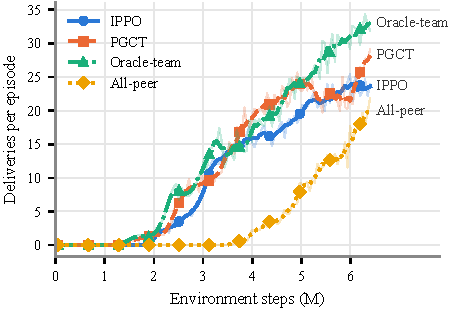
\includegraphics[width=\columnwidth]{figures/fig1_learning_curves.pdf}
\caption{E1의 평가 배송 수/episode(seed 1개\pilot). 가는 선: 원 평가값, 굵은 선: 중심 5점 이동평균.}
\label{fig:curves}
\end{figure}

\textbf{E1의 학습.} \ours{}는 모든 지표에서 독립 학습보다 나았다(표~\ref{tab:e1}, 그림~\ref{fig:curves}).\pilot{} episode당 배송 1개에 0.26M step 먼저 도달했고, 평균 처리량
12\%, 최종 처리량 18\%가 높았으며, episode당 20개에 가장 먼저 도달했다(4.15M; Oracle-team 4.66M, IPPO 5.07M). All-peer는 시작을 약 2백만 step 늦췄다. agent별로 보면(부록 D)
IPPO는 팀당 한 명만 배송을 배웠고, \ours{}와 Oracle-team은 세 번째 agent를, All-peer는 늦었지만 네 명 모두를 학습시켰다. 유능한 동료의 critic을 distillation하면 자기 보상을
거의 받지 못하는 agent에게 학습 신호가 생긴다는 가설을 세운다. 이를 검증하려면 해당 agent로의 전이를 차단하는 개입 실험이 필요하다 \todo{개입 실험}.

\begin{figure*}[t]
\centering
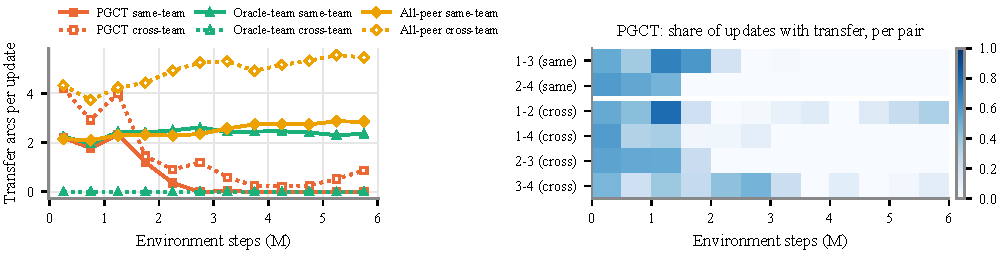
\includegraphics[width=\textwidth]{figures/fig3_critic_transfer.pdf}
\caption{E1의 실제 critic 전이(seed 1개\pilot). 왼쪽: update당 방향성 전이 arc 수, 팀 안(실선)과 팀 간(점선), 0.5M step 구간. 오른쪽: \ours{}에서 각 쌍이 critic 정보를 주고받은
update 비율.}
\label{fig:transfer}
\end{figure*}

\textbf{E1의 추론은 분석과 일치한다.} 명제~\ref{prop:nonid}는 E1에서 팀을 식별할 수 없다고 예측한다. 실제로 2.5M step 이후 거의 모든 checkpoint와 모든 방법에서 팀원 사이
probe divergence가 팀원이 아닌 쌍보다 컸다(부록 D). 즉 실측 마진이 음수였고, v2 추론 집합을 포함한 probe 부분집합 5개에서 고정 모델로 재도 같았다. 따라서 \ours{}는 팀을
복원하지 못했다. 4M step 이후 전이 arc의 95\%가 다른 팀 agent를 이었고(update당 0.03 대 0.63 arc; 그림~\ref{fig:transfer}), 연결된 쌍은 같은 역할(자기 구역에 머묾 / 상대
구역에서 선반을 가져옴)의 agent였다. 따라서 성능 향상에는 세 설명이 가능하다. 팀원 간 전이(H1), 팀과 무관하게 행동이 비슷한 agent 간 선택적 전이(H2), 단순히 All-peer보다
적은 전이(H3; \ours{}는 2M step 이후 update의 29--37\%에서 전이, All-peer는 거의 전부). E1 데이터는 H1을 원인에서 배제한다. 전이량을 맞춘 random gate가 H2와 H3를 가를 것이다
\todo{random gate}. H2와 일관되게, 별도의 고정 평가에서 receiver의 critic을 팀원이 아닌 agent와 섞을 때가 팀원과 섞을 때보다 가치 오차를 더 줄였다(같은 팀 AUROC
0.25--0.33). 따라서 여기서 팀 간 연결은 해롭지 않았다.

\textbf{목표가 분리된 팀(E1-F).} \todo{채울 것: (1) Oracle-team 대 All-peer; (2) 팀 내 대 팀 간 호환성; (3) \ours{}와 \ours{}-v2의 $\hat{\mathcal{T}}_i$ 정밀도·재현율, AUROC,
$\Delta$와 $\rho$; (4) IPPO, All-peer, Random-gated, Oracle-team 대비 학습.}

\begin{table}[t]
\centering
\small
\resizebox{\columnwidth}{!}{%
\begin{tabular}{lcccccc}
\toprule
방법 & 시작 & 평균 & 최종 & 정밀도 & 재현율 & $\Delta$ \\
\midrule
IPPO & \tbd & \tbd & \tbd & -- & -- & \tbd \\
All-peer & \tbd & \tbd & \tbd & \tbd & \tbd & \tbd \\
Random-gated & \tbd & \tbd & \tbd & \tbd & \tbd & \tbd \\
\ours{} & \tbd & \tbd & \tbd & \tbd & \tbd & \tbd \\
\ours{}-v2 & \tbd & \tbd & \tbd & \tbd & \tbd & \tbd \\
Oracle-team & \tbd & \tbd & \tbd & 1 & 1 & \tbd \\
\bottomrule
\end{tabular}}
\caption{E1-F(목표 분리). 실제 update에서 추론한 국소 팀 관계의 정밀도와 재현율; $\Delta$: probe divergence의 실측 분리 마진. \todo{실행이 끝나면 채움}}
\label{tab:e1f}
\end{table}

\section{논의와 한계}
\textbf{분석이 주는 것과 주지 않는 것.} 명제~\ref{prop:recovery}--\ref{prop:bias}는 ``비슷한 행동 $\Rightarrow$ 같은 팀 $\Rightarrow$ 유용한 critic''이라는 비형식적 사슬을
확인 가능한 조건으로 바꾼다. 양의 마진, 작은 변화량, 호환되는 팀원 가치다. 명제~\ref{prop:counter}와 \ref{prop:nonid}는 첫째와 둘째 고리가 실패할 수 있음을 보이며, E1은 둘째 실패의
사례다. 결합된 학습 동역학의 수렴은 보장하지 않는다.

\textbf{팀 발견인가 호환성 발견인가.} 설계자가 존중하고 싶은 것이 흔히 팀 관계이므로 우리의 목표는 팀원 추론(Q1)이다. 팀을 식별할 수 없거나 호환성이 팀 소속을 따르지 않을 때는
전이 효용을 직접 겨냥하는 gate(Q2)가 더 일반적인 목표다. 이때 probe divergence는 유용성을 측정해야 하는 대리 지표로 읽을 수 있다. 예를 들어 $D_{ij}$와 추정한
$U_{i\leftarrow j}$ 사이의 순위 상관으로 측정한다.

\textbf{가정과 범위.} \ours{}는 가정~\ref{as:comparability}를 만족하는 공유 probe 집합이 필요하다. 우리 집합은 맵 배치에서 고정 규칙으로 구성하며, probe 민감도(개수, 설계,
무작위 probe)를 보고해야 한다 \todo{probe ablation}. 관측에 agent 위치가 있으면 이처럼 단일 step·0 상태 probe로 충분하고, 그렇지 않으면 이력이 필요할 수 있다. 공통 어휘가
있다면 agent들이 팀 식별자를 교환할 수 있다. 팀원 추론은 목표가 비공개이거나 라벨이 공유되지 않을 때 의미가 있다. agent 4명, 팀 2개의 한 환경 계열을 평가했고, E1 결과는 seed
1개다. 같은 seed를 다시 실행하면 IPPO는 정확히 재현됐지만 공유 방식은 그렇지 않았다(부록 D).

\section{결론}
우리는 공유 probe 집합에 대한 응답으로 국소 팀원을 추론하고 그 critic을 distillation하는 Probe-Gated Critic Transfer를 연구했다. 이것이 정당한 조건(분리, 유계 변화량, 호환되는 가치)을
명시하고 실패하는 경우를 보였으며, 결정 문제가 일치하는 팀에 대한 식별 불가능성 결과도 포함했다. 이런 팀 대칭 과제에서 \ours{}는 예측대로 팀을 복원하지 못했지만 예비 실행에서
학습을 개선했다. 조건이 성립할 때 팀을 복원하고 도움이 되는지는 목표 분리 과제에서 평가 중이다.

\bibliographystyle{plainnat}
\bibliography{references}

\clearpage
\appendix
\onecolumn

\section{증명}

\textbf{명제~\ref{prop:properties}.}
(a) $m=\frac{p+q}{2}$에 대해 $\KL(p\Vert m)=\sum_a p(a)\ln\frac{2p(a)}{p(a)+q(a)}\le\sum_a p(a)\ln 2=\ln 2$이고 $q$도 같다. 따라서 $0\le\JS\le\ln2$이다. 대칭은 자명하다.
$\JS(p,q)=0$은 $\KL(p\Vert m)=\KL(q\Vert m)=0$, 즉 $p=m=q$와 동치다. probe에 대한 평균은 세 성질을 보존하며, 0이 되는 것은 모든 항이 0일 때뿐이다.
(b) $\JS(p,q)=\sum_a q(a)\,\phi\!\big(p(a)/q(a)\big)$, $\phi(t)=\frac{t}{2}\ln\frac{2t}{1+t}+\frac12\ln\frac{2}{1+t}$이며 $\phi$는 볼록이고 $\phi(1)=0$이다. 따라서 $\JS$는
$f$-divergence이고, $f$-divergence는 두 인자에 대해 결합 볼록이다(볼록 함수의 perspective). 서로 다른 좌표의 결합 볼록 함수의 합은 결합 볼록이다.
(c) $\sqrt{\JS}$는 $\Delta(\mathcal{A})$ 위의 metric이다~\cite{endres2003metric}. $x_m=\sqrt{\JS(p_i^m,p_k^m)}$, $y_m=\sqrt{\JS(p_i^m,p_j^m)}$, $w_m=\sqrt{\JS(p_j^m,p_k^m)}$이면
$x_m\le y_m+w_m$이고, Minkowski 부등식으로 $\big(\frac1M\sum_m x_m^2\big)^{1/2}\le\big(\frac1M\sum_m y_m^2\big)^{1/2}+\big(\frac1M\sum_m w_m^2\big)^{1/2}$, 즉 $d_{ik}\le d_{ij}+d_{jk}$이다.
대칭과 $d_{ii}=0$은 (a)에서 나온다. $\mathcal{Q}$에서 일치하는 정책은 $d=0$이므로 pseudometric이다.

\textbf{명제~\ref{prop:recovery}.} $z_i=z_j$이면 $\bar D_{ij}\le D_{ij}+\epsilon\le\delta_{\mathrm{in}}+\epsilon<\tau$이므로 $j\in\hat{\mathcal{T}}_i$이다. $z_i\ne z_j$이면
$\bar D_{ij}\ge D_{ij}-\epsilon\ge\delta_{\mathrm{out}}-\epsilon>\tau$이므로 $j\notin\hat{\mathcal{T}}_i$이다. $\tau$의 구간이 비어 있지 않을 조건은 $2\epsilon<\Delta$다. 조건이 $i$와 $j$의
순서에 의존하지 않으므로 대칭이다.

\textbf{보조정리~\ref{lem:drift}.} KL의 결합 볼록성으로 $\KL(p\Vert\frac{p+p'}{2})\le\frac12\KL(p\Vert p)+\frac12\KL(p\Vert p')=\frac12\KL(p\Vert p')$이고, 마찬가지로
$\KL(p'\Vert\frac{p+p'}{2})\le\frac12\KL(p'\Vert p)$이다. 따라서 $\JS(p,p')\le\frac14(\KL(p\Vert p')+\KL(p'\Vert p))\le\kappa/4$다. 각 probe에서 $\sqrt{\JS}$의 삼각부등식으로
$|\sqrt{\JS(p_i'^m,p_j'^m)}-\sqrt{\JS(p_i^m,p_j^m)}|\le\sqrt{\JS(p_i^m,p_i'^m)}+\sqrt{\JS(p_j^m,p_j'^m)}\le\sqrt{\kappa}$이다. probe에 대한 Minkowski 부등식으로
$|d'_{ij}-d_{ij}|\le\sqrt{\kappa}$이고, 명제~\ref{prop:properties}(a)에 의해 $|D'-D|=|d'-d|(d'+d)\le\sqrt{\kappa}\cdot2\sqrt{\ln 2}$이다.

\textbf{명제~\ref{prop:tracking}.} $e_n=\bar D(n)-D(n)$이라 하면 $e_n=(1-\beta)\bar D(n-1)+\beta D(n)-D(n)=(1-\beta)e_{n-1}+(1-\beta)(D(n-1)-D(n))$이므로
$|e_n|\le(1-\beta)|e_{n-1}|+(1-\beta)\rho$이다. 첫 측정으로 초기화하면 $e_1=0$이므로 $|e_n|\le(1-\beta)\rho\sum_{k\ge0}(1-\beta)^k=\frac{1-\beta}{\beta}\rho$이다.

\textbf{명제~\ref{prop:bias}.} $f''(v)=2c+2\lambda\sum_j\alpha_{ij}=2(c+\lambda)$이므로 $f$는 $2(c+\lambda)$-강볼록이고 유일한 정류점 $v^\star$를 가진다. 그러면
$v^\star-y=\frac{\lambda}{c+\lambda}\sum_j\alpha_{ij}(v_j-y)$이고, $|v_j-y|$의 한계와 삼각부등식으로 결과를 얻는다.

\textbf{명제~\ref{prop:counter}.} 상태 하나, 행동 하나, $\mathcal{Q}=\{q\}$이고 두 agent의 정책이 그 행동의 점질량이면 $D_{ij}=0$이다. $r_i\equiv0$, $r_j\equiv1$이면 $V_i=0$,
$V_j=\sum_t\gamma^t=1/(1-\gamma)$이다.

\textbf{명제~\ref{prop:nonid}.} 다른 agent를 고정하면, 기억 없는 사상 $\mu$의 agent $i$에 대한 기대 할인 return은 $i$가 $\mu$ 아래에서 겪는 관측--보상 열 분포의 범함수다. 서로 다른
팀의 $i$와 $j$에 대해 모든 $\mu$에서 이 분포가 일치하면 모든 $\mu$의 return이 같으므로 최적 사상의 집합이 일치한다. 최적 사상 $\mu^\star$가 유일하면 모든 목표 최적 정책은 모든
관측(모든 probe 포함)에서 $\mu^\star$와 같으므로 $p_i^m=p_j^m$이고 모든 쌍에서 $D_{ij}=0$이다. 그러면 $\delta_{\mathrm{in}}=\delta_{\mathrm{out}}=0$, $\Delta=0$이고
$\delta_{\mathrm{in}}<\tau\le\delta_{\mathrm{out}}$을 만족하는 $\tau$는 없다.

\section{하이퍼파라미터}
\begin{table}[h]
\centering
\small
\begin{tabular}{ll}
\toprule
Setting & Value \\
\midrule
Map / agents / teams & 11$\times$10 E1 / 4 / 2 \\
Reward & individual \\
Home-zone shelf ratio & 0.5 \\
Requests per team & 2 \\
Sensor / communication range & 5 / 5 \\
Learning rate & 0.0002 \\
Entropy coef. & 0.05 \\
$\gamma$ / GAE $\lambda$ & 0.99 / 0.95 \\
Rollout / BPTT length & 1024 / 64 \\
PPO epochs / minibatches / clip & 4 / 8 / 0.2 \\
Hidden (MLP / GRU) & 128 / 128 \\
Peer-loss coef. $\lambda_{peer}$ & 0.01 \\
Gate: JS threshold / EMA $\beta$ / warm-up & 0.12 / 0.35 / 100 upd. \\
Canonical probes & 48 (fixed, zero hidden, length 1) \\
Evaluation & every 50 updates, 20$\times$500 steps, deterministic \\
\bottomrule
\end{tabular}

\caption{처음부터 학습한 E1 비교의 설정(donor 집합을 제외하고 모든 방법이 동일).}
\end{table}

\section{구간별 실제 전이}
\begin{table}[h]
\centering
\small
\begin{tabular}{llccc}
\toprule
Method & Window & Updates w/ transfer & Same-team arcs/upd. & Cross-team arcs/upd. \\
\midrule
PGCT & 0--2.0M & 91\% & 1.86 & 3.09 \\
 & 2--4.0M & 37\% & 0.10 & 0.73 \\
 & 4--6.4M & 29\% & 0.03 & 0.63 \\
\addlinespace
Oracle-team & 0--2.0M & 82\% & 2.26 & 0.00 \\
 & 2--4.0M & 86\% & 2.50 & 0.00 \\
 & 4--6.4M & 85\% & 2.39 & 0.00 \\
\addlinespace
All-peer & 0--2.0M & 99\% & 2.22 & 4.18 \\
 & 2--4.0M & 100\% & 2.49 & 5.10 \\
 & 4--6.4M & 100\% & 2.79 & 5.37 \\
\bottomrule
\end{tabular}

\caption{E1의 학습 구간별 실제 전이(seed 1개). arc는 receiver--donor 방향 연결이다.}
\end{table}

\section{추가 E1 결과}
\begin{figure}[h]
\centering
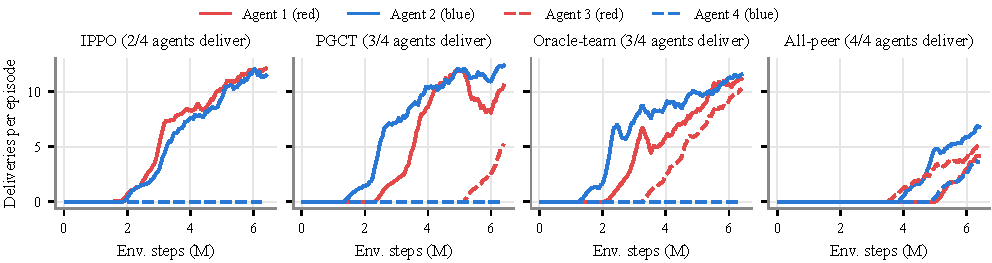
\includegraphics[width=\textwidth]{figures/fig2_per_agent_deliveries.pdf}
\caption{E1의 agent별 배송 수/episode(5점 이동평균, seed 1개). 빨강: 빨강 팀(agent 1, 3), 파랑: 파랑 팀(agent 2, 4), 실선: agent 1--2, 점선: agent 3--4.}
\end{figure}
\begin{figure}[h]
\centering
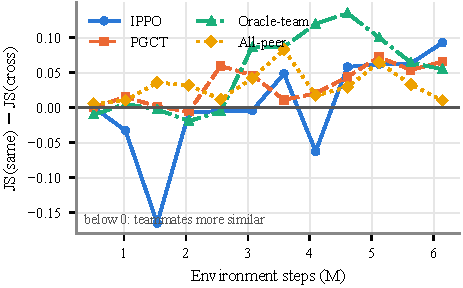
\includegraphics[width=0.6\textwidth]{figures/fig4_probe_js_gap.pdf}
\caption{E1 checkpoint에서 팀원 사이 probe divergence에서 팀원이 아닌 쌍의 값을 뺀 것(seed 1개). 0보다 크면 팀원이 더 다르다. 즉 실측 마진이 음수다.}
\end{figure}
\begin{figure}[h]
\centering
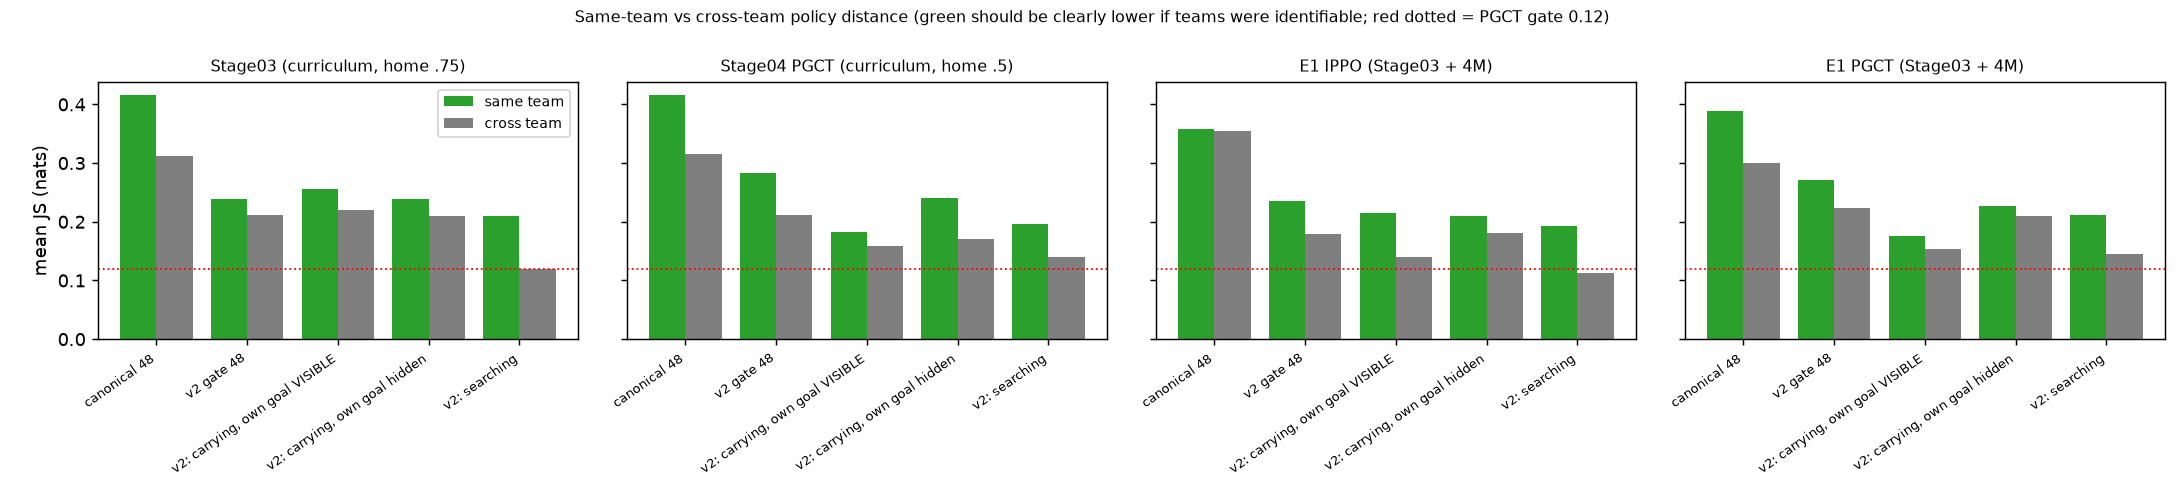
\includegraphics[width=\textwidth]{figures/frozen_probe_same_vs_cross.png}
\caption{고정 E1 모델 4개와 probe 부분집합 5개(v2 추론 집합 포함)에서 팀원(초록)과 팀원이 아닌 쌍(회색)의 평균 probe divergence. 20개 조합 모두에서 팀원이 덜 비슷하다. 빨간 점선:
$\tau=0.12$.}
\end{figure}
\begin{figure}[h]
\centering
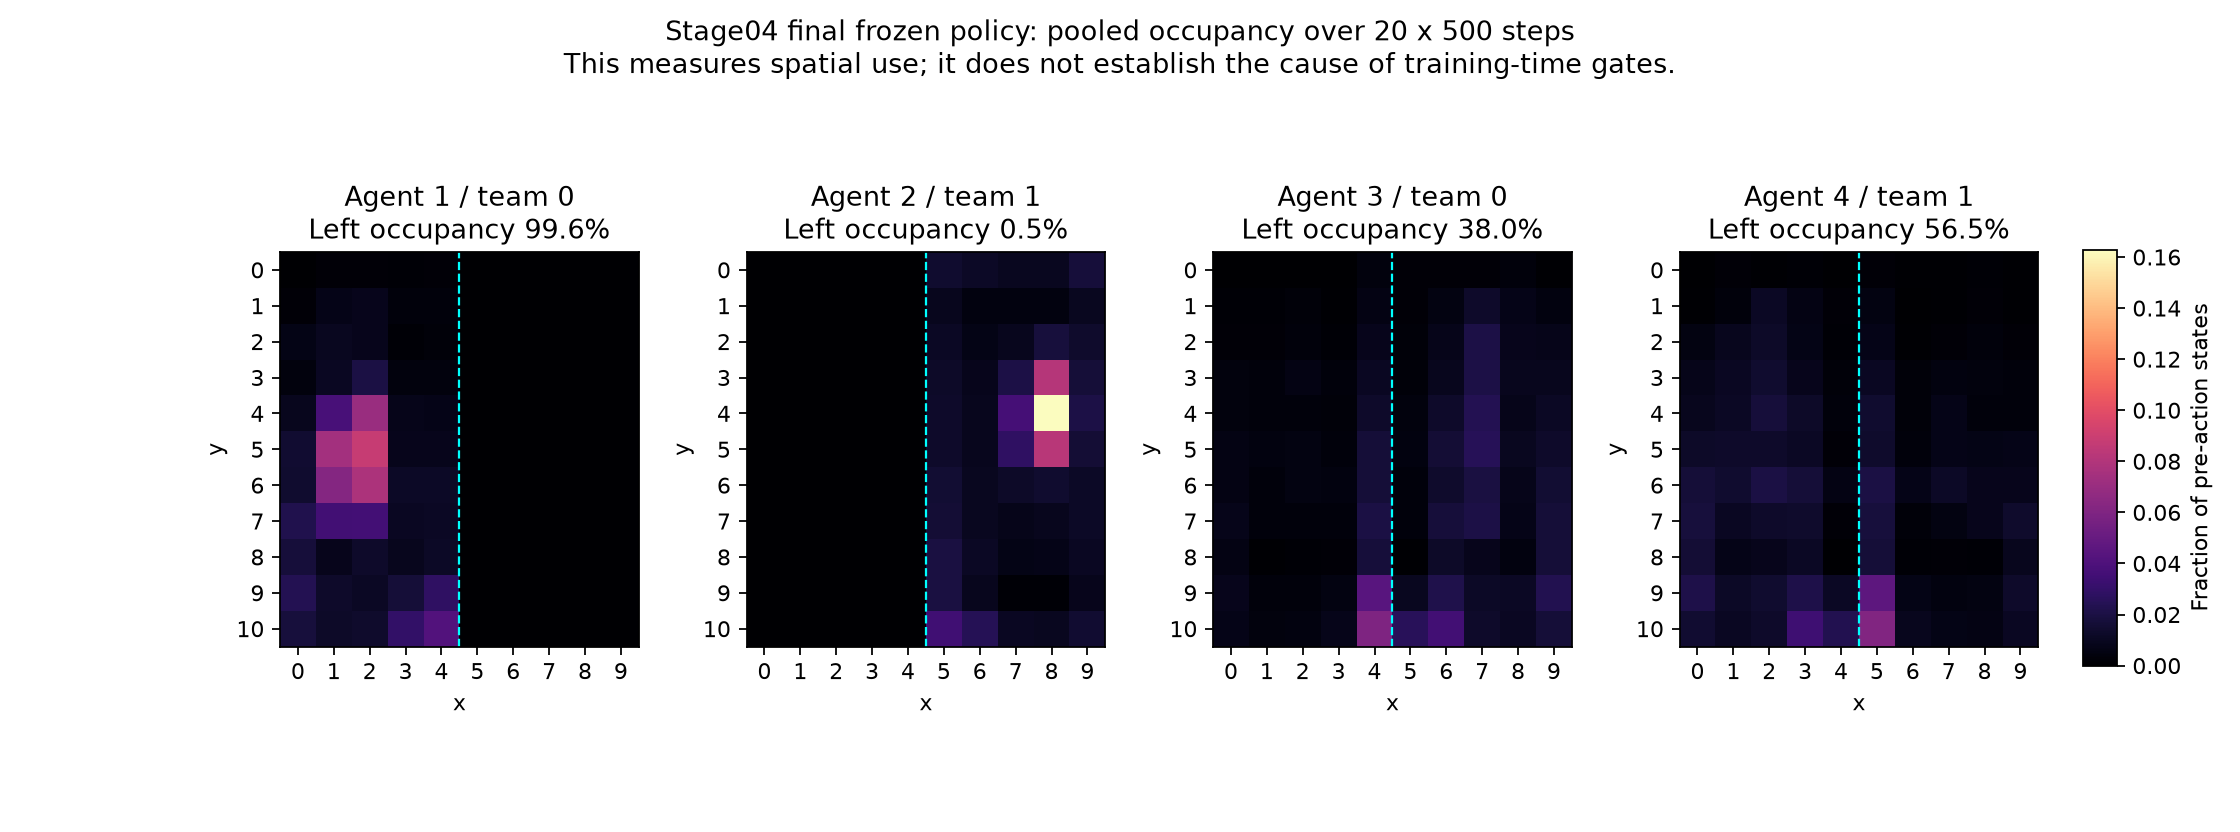
\includegraphics[width=\textwidth]{figures/stage04_occupancy.png}
\caption{고정 커리큘럼 모델(선반의 50\%를 상대 팀 구역에 배치)의 칸 점유. agent 1과 2는 자기 팀 구역에 머물고, agent 3과 4는 상대 구역에서 선반을 가져오며 gate가 가장 자주 연결한 쌍이다.}
\end{figure}
\begin{figure}[h]
\centering
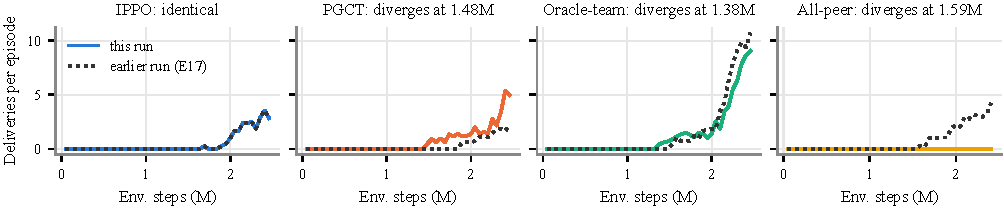
\includegraphics[width=\textwidth]{figures/figA1_reproducibility.pdf}
\caption{같은 seed와 초기 가중치의 두 실행(실선: 보고한 실행, 점선: 이전에 중단된 실행). IPPO는 정확히 재현되고, 공유 방식은 1.4--1.6M step 이후 갈라진다.}
\end{figure}

\end{document}
